\begin{frame}
    \frametitle{Frequency Deviation}
    % Talk about the wacky result from sample D around 0.17, what's doing 
    \begin{columns}
            \column[t]{5cm}
            \begin{figure}
                    \begin{center}
                            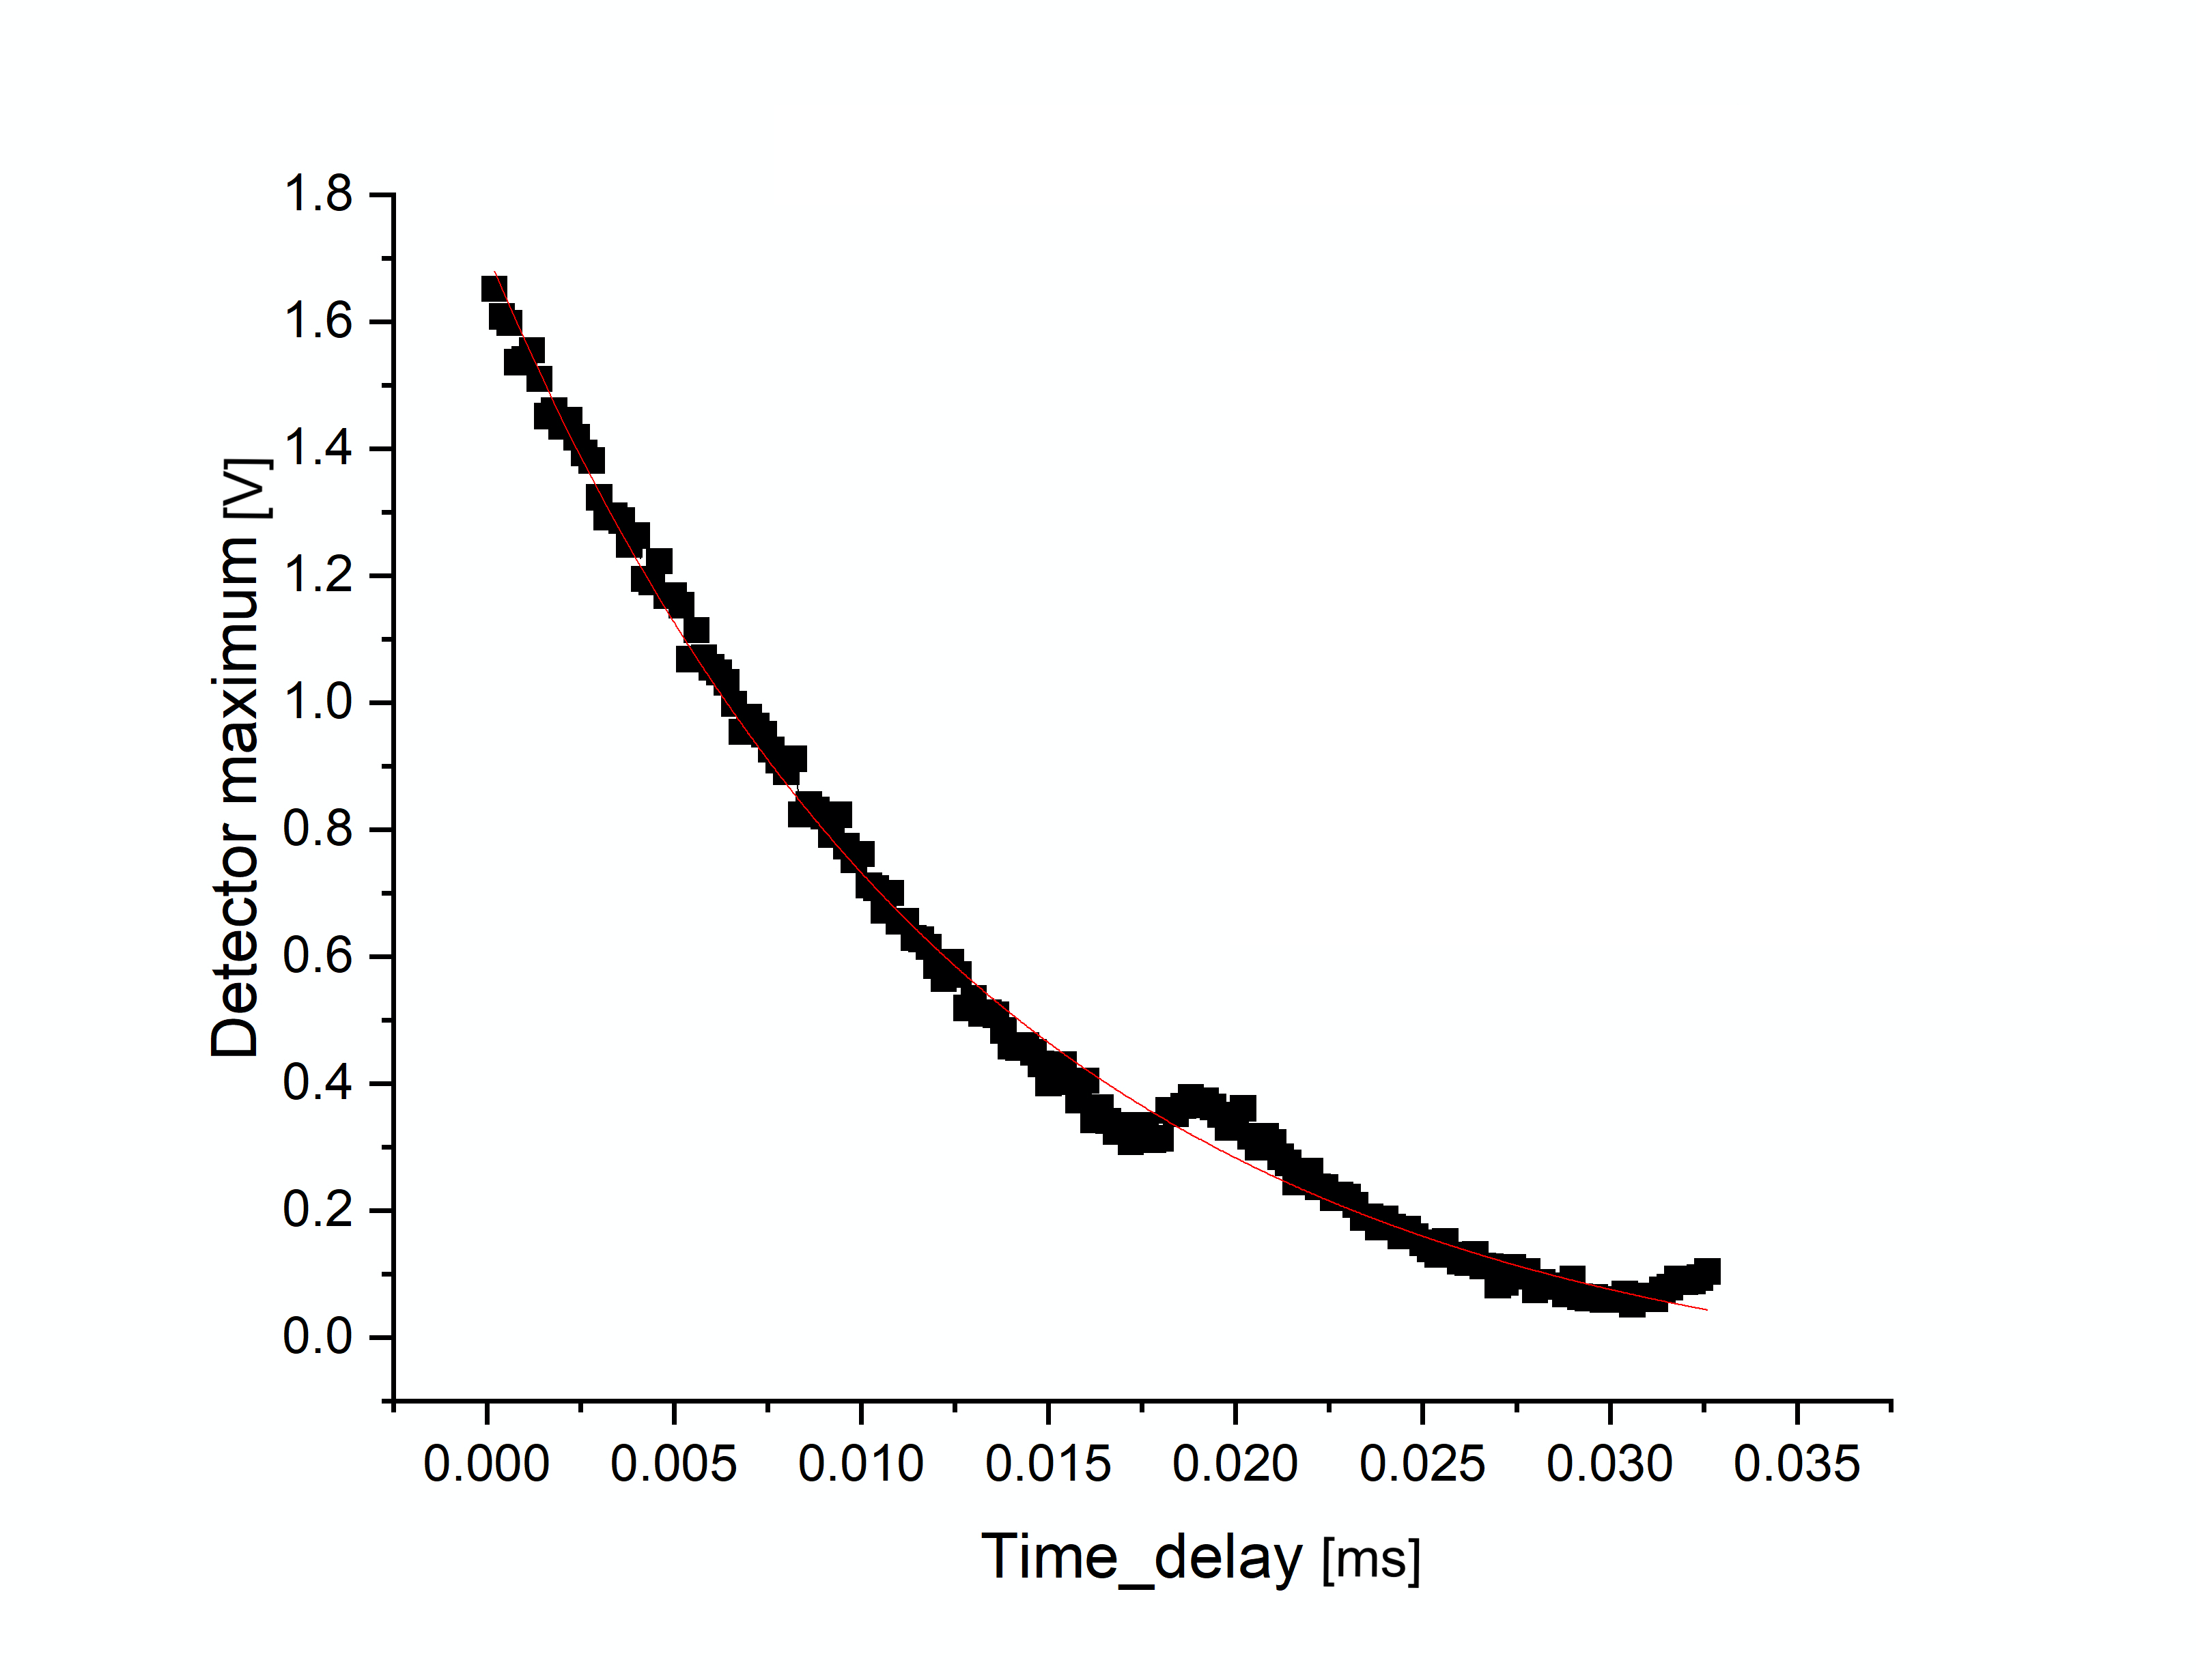
\includegraphics[height=3cm]{./images/figures/theory/d-t1.png}
                    \end{center}
                            \caption{Sample D [$ 3.37 \pm 1.6 x 10^{-2}$]:$ T_1$}
                    \label{fig:d_t1}
            \end{figure}
            \column[t]{5cm}
            \begin{figure}[htbp!]
                    \begin{center}
                            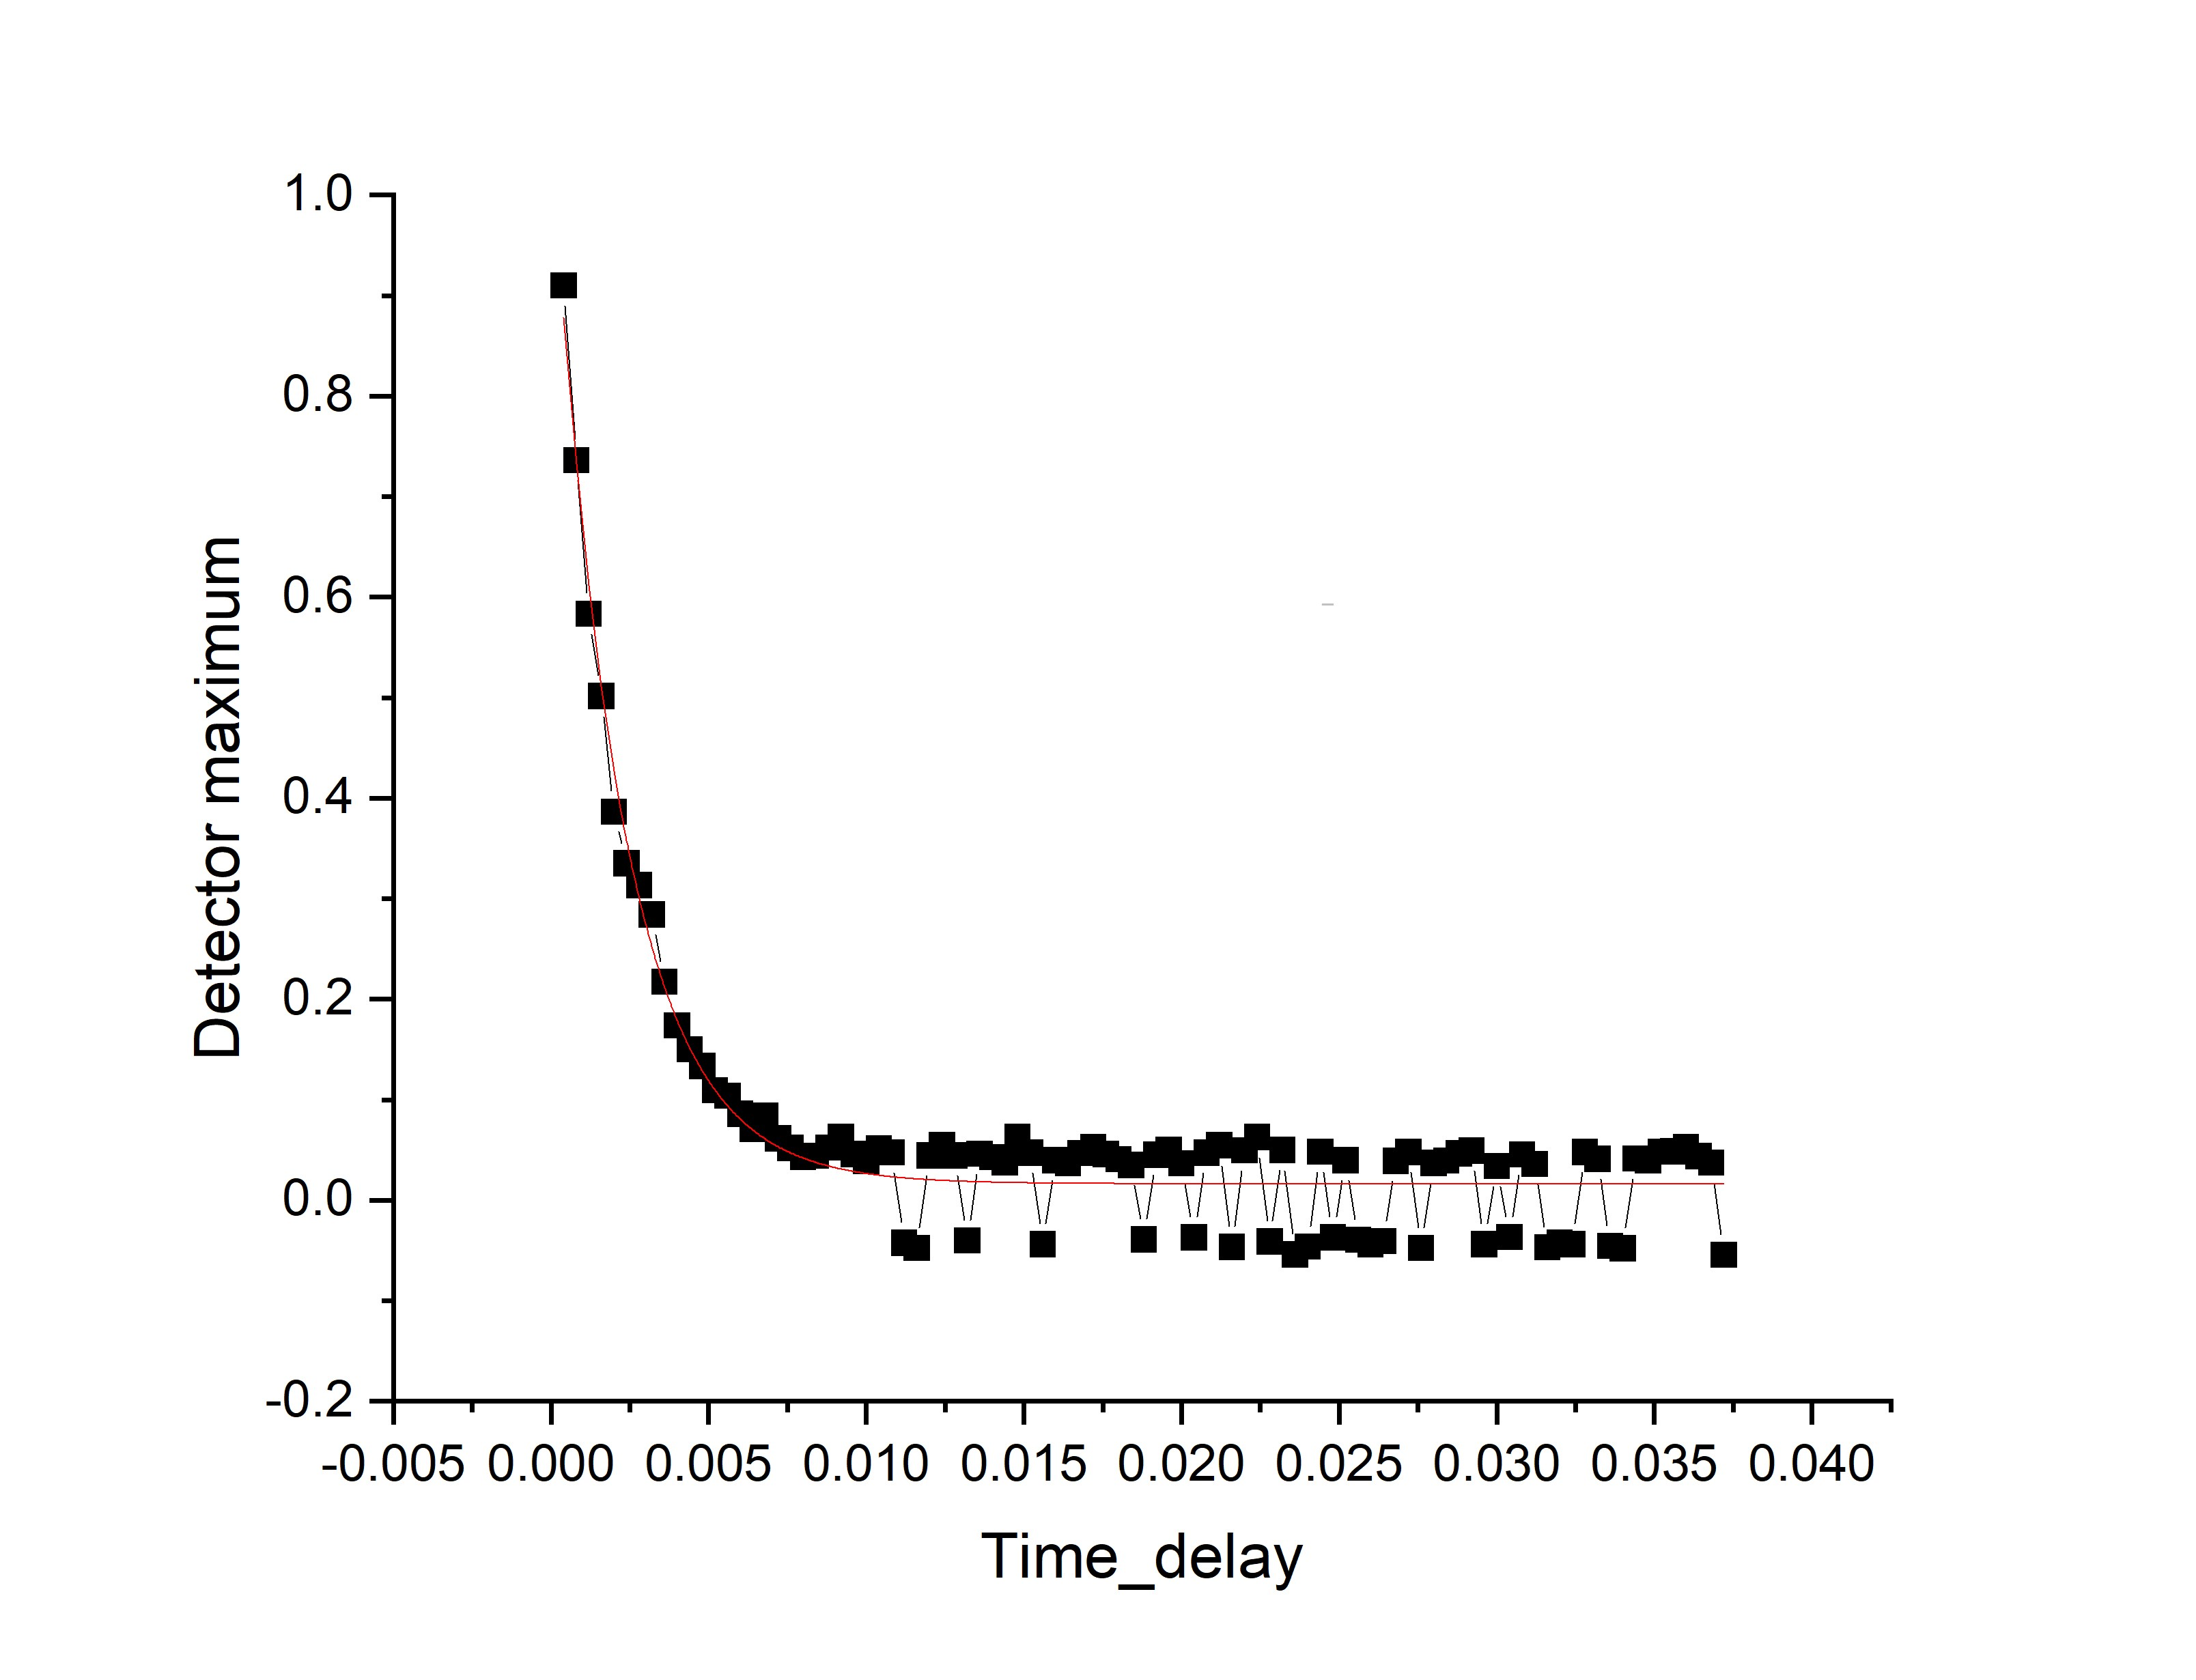
\includegraphics[height=3.06cm]{./images/figures/t_plots_appendix/h_t2.jpg}
                    \end{center}
                            \caption{Sample H [$ 53.3 \pm 8.1 x 10^{-2}]$: $T_2$}
                    \label{fig:h_t2}
            \end{figure}
          \end{columns}
\end{frame}